% !TEX root = ./../../_Thesis.tex

% section's Name and Label
\section{Validation}}
\label{sec:Validation}

To validate the visual simulation results of the refractive errors, we use DSLR camera (Canon model EOS Rebel T3 with 18-55mm lens). The camera represents a perfect eye (\ie without refractive aberrations). We place additional lenses in front of the camera's optical system to induce low-order aberrations (\ie, myopia, hyperopia, and astigmatism). Such lenses are placed on a support fixed to a UV filter attached to the main lens. Figure~\ref{fig:extralens} shows the camera with an external +1.0 diopter lens attached to it. The support can hold up to three additional lenses. 
%
%results from the image filtering process, we've used additional lenses to induce low-order aberrations (\ie, myopia, hyperopia, and astigmatism) into the DSLR camera's optical system (Figure~\ref{fig:extralens}). 
We have also created a synthetic eye model and adjusted it according to the camera's configuration to achieve consistent results.
% with the ones captured by the camera. 
When comparing results, we make sure that the \emph{f-number} (\ie, the ratio of the lens' focal length $f$ to the diameter $D$ of the entrance pupil):
\begin{equation}
	\centering
	\label{eq:fnumber}
	f_{number} = \frac{f}{D}
\end{equation}
\noindent
is the same for the optical systems of both the camera and the synthetic eye. For the experiments, we setup the focal length of the camera's main lens to 18mm (regardless of the use or not of additional lenses).
% to captured images (with or without extra lenses) with 18mm focal length and 
Thus, for \emph{f-number} values of $4.0$, $4.5$ and $5.0$, the camera lens aperture would be
%entrance pupil for each possible combination is
 4.5mm, 4.0mm and 3.6mm, respectively. 
Our synthetic eye model (Figure~\ref{fig:syntheticeye}) has a diameter of 18mm. Due to the presence of the crystalline lens,  its actual focal length of 13.5mm: $f_{eye} = 18mm \times \eta_{eye} =  18mm \times 1.333 = 13.5 mm$, where $\eta_{eye}$ is the index of refraction of the eye. As a result, for the simulations, the pupil size (equivalent of the camera's lens aperture) needs to be rescaled to maintain the same \emph{f-number} values as the camera. Table~\ref{table:pupildiameter} shows the corresponding values of the equivalent camera apertures and pupil diameters. The simulation results shown in \review{Chapter~\ref{chap:Results}} were obtained for $f/5.0$.

%we must rescale the entrance pupil's diameter (Table~\ref{table:pupildiameter}) in order to maintain the same \emph{f-number} in simulations of retinal images. 

\begin{table}[h]
	\centering
	\caption{Camera apertures and pupil diameters for various f-numbers.}
	\label{table:pupildiameter}
	\begin{tabular}{rcc}
		\multicolumn{1}{l}{\bf f-number} & {\bf DSLR Camera (18mm focal length)} & {\bf Synthetic Eye (13.5mm focal length)} \\
		{\bf }               & {\bf aperture}     & {\bf pupil diameter}     \\
		{\bf $f/4.0$}         & 4.5mm                    & 3.4mm                        \\
		{\bf $f/4.5$}         & 4.0mm                    & 3.0mm                        \\
		{\bf $f/5.0$}         & 3.6mm                    & 2.7mm                        
	\end{tabular}
\end{table}

\begin{figure}[h]
	\centering
	
	\subfigure[]{
		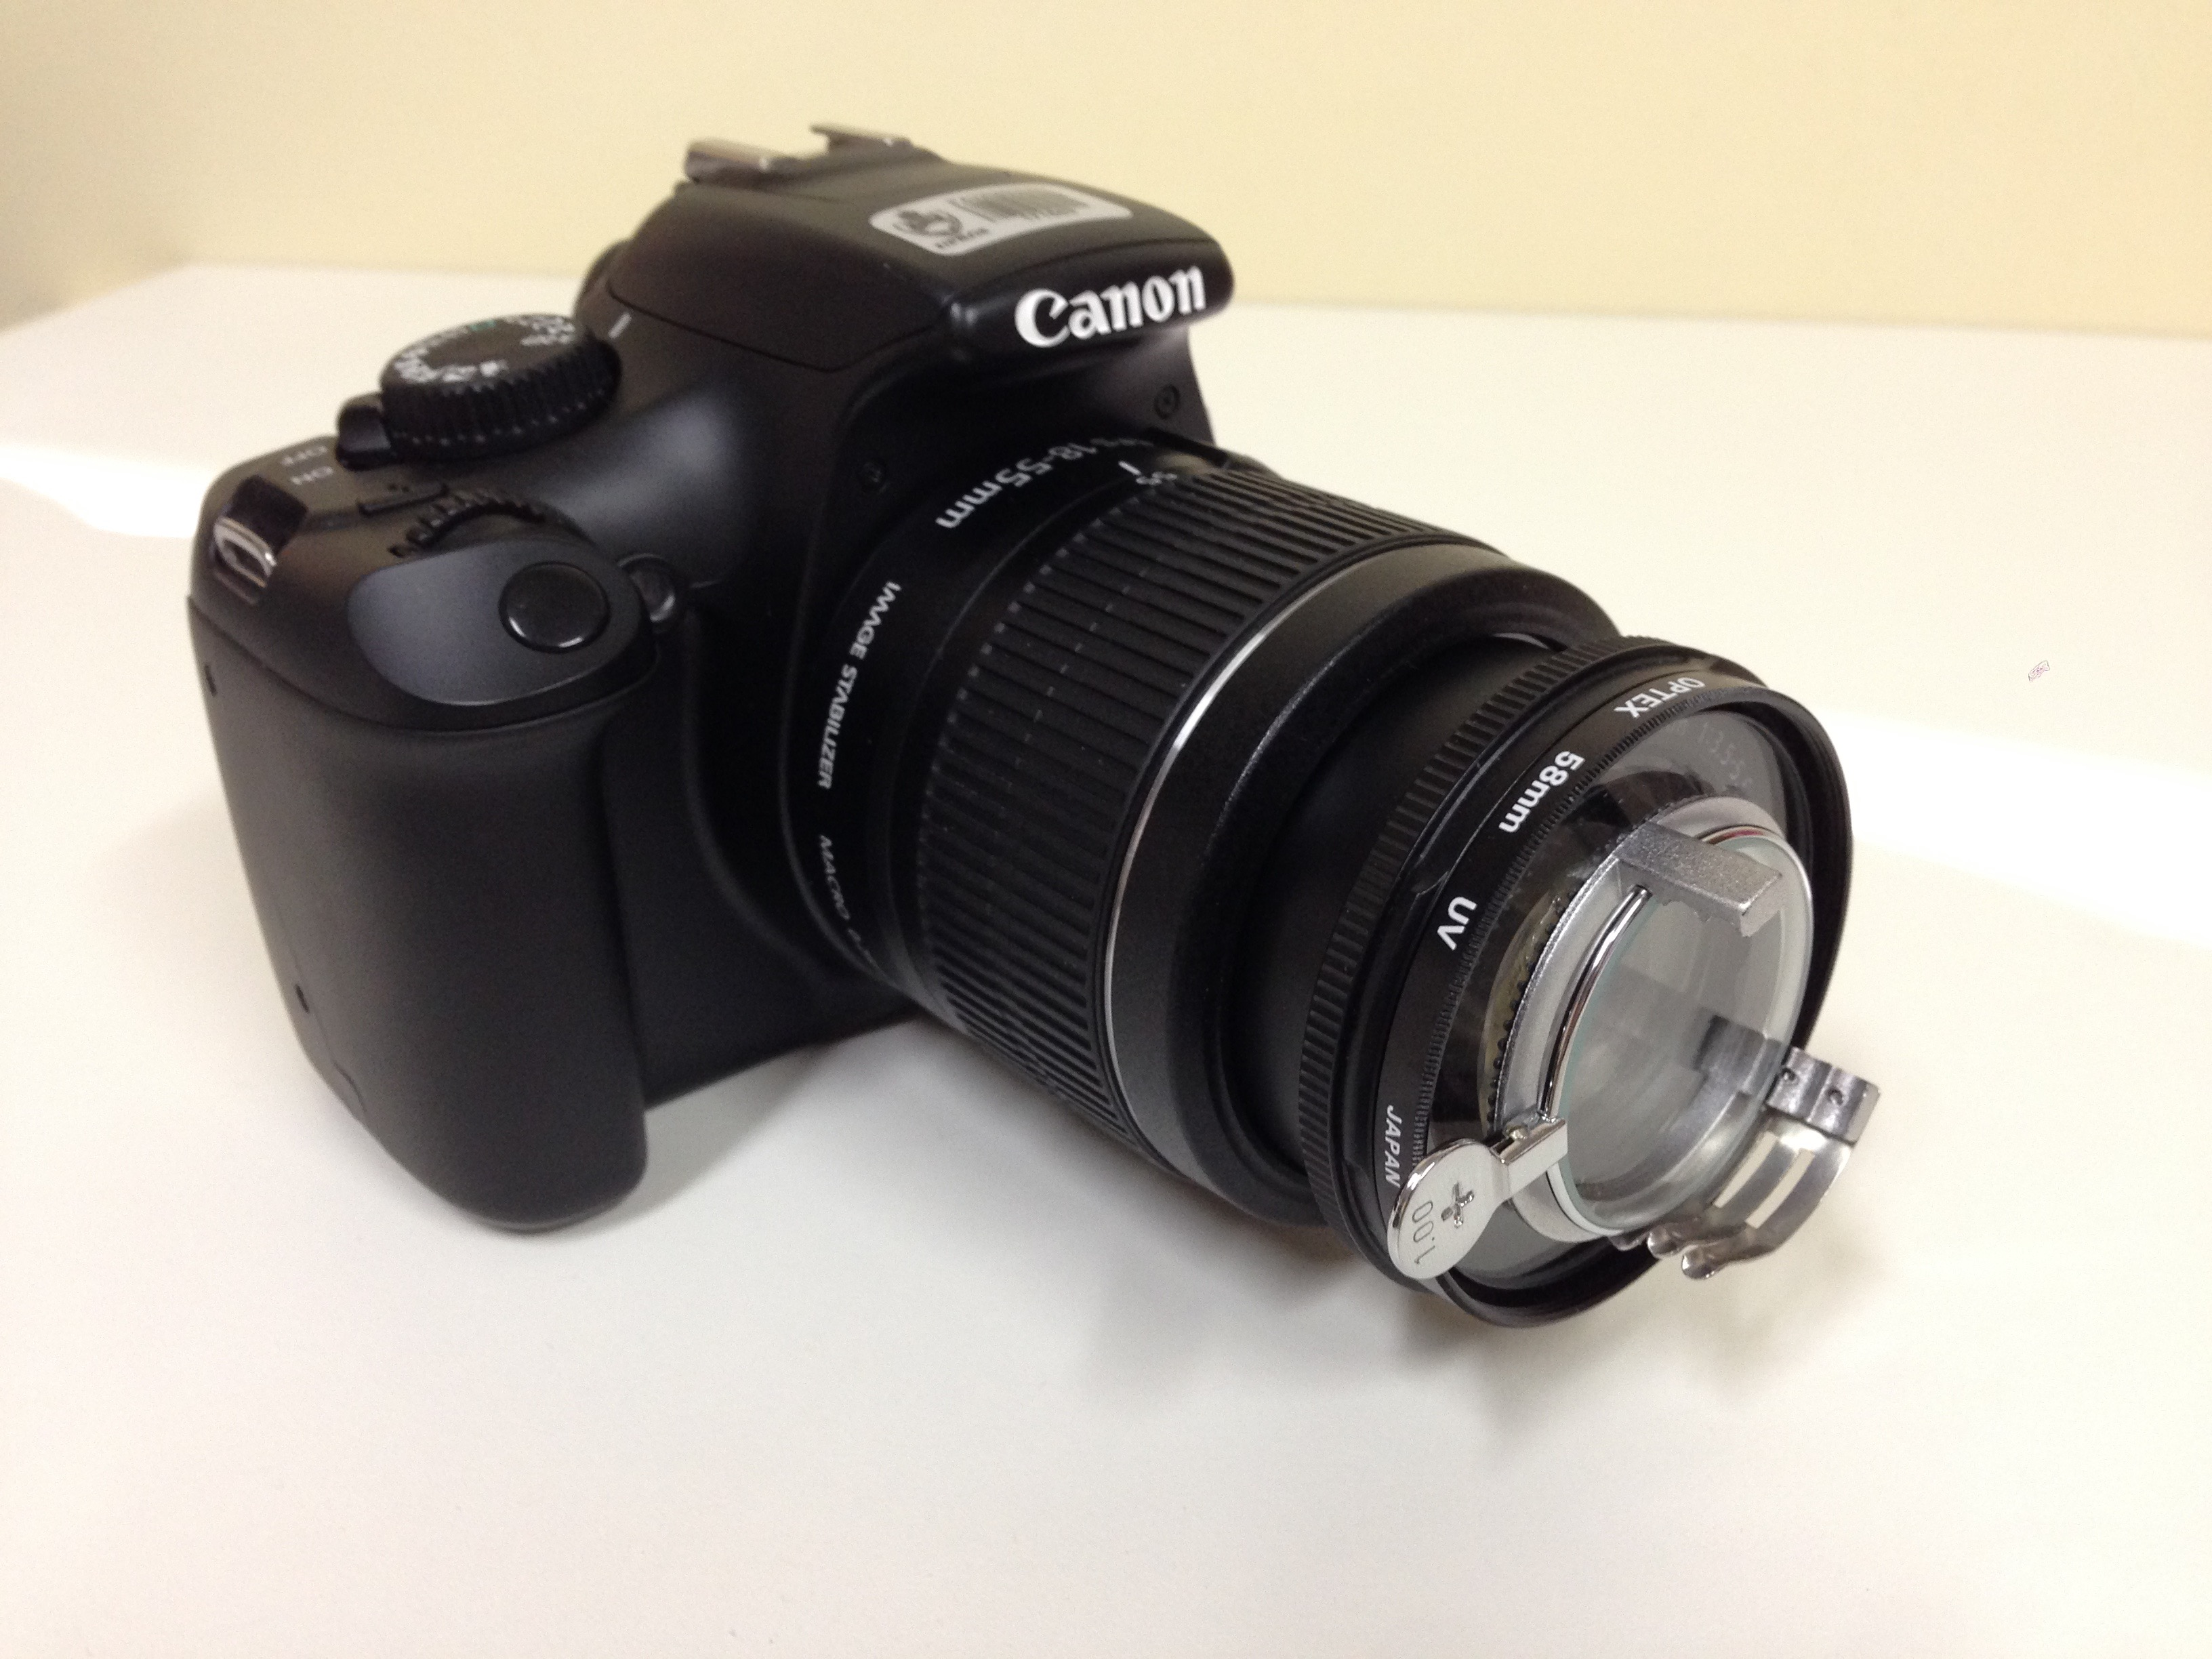
\includegraphics[width=0.55\linewidth]{__Images/04/camera.jpg}
		\label{fig:extralens}
	}
	~
	\subfigure[]{
		
\includegraphics[width=0.35\linewidth]{__Images/04/eyemodel.png}
		\label{fig:syntheticeye}
	}
	
	\caption[Optical systems used in the validation process]{Optical systems used in the validation process: (a) Canon EOS Rebel T3 with apparatus to add up to three extra lenses. Focal lens set to 18mm; (b) synthetic eye model with effective focal length of 13.5mm.}
	\label{fig:camera}
\end{figure}